\documentclass[border=10pt]{standalone}
\usepackage[T1]{fontenc}
\usepackage{amsmath,amsfonts}
\usepackage{tikz}
\usetikzlibrary{shapes.geometric} % Cylinder
\usetikzlibrary{shadows.blur,arrows.meta,bending,positioning,mindmap,trees}
\usetikzlibrary{%
	calc,%
	decorations.pathmorphing,%
	fadings,%
	shadings,
   decorations.pathreplacing,calligraphy
}
\usepackage{xcolor}
\makeatletter% from https://tex.stackexchange.com/a/39698/121799
\def\grd@save@target#1{%
  \def\grd@target{#1}}
\def\grd@save@start#1{%
  \def\grd@start{#1}}
\tikzset{
  labeled grid/.style={
    to path={%
      \pgfextra{%
        \edef\grd@@target{(\tikztotarget)}%
        \tikz@scan@one@point\grd@save@target\grd@@target\relax
        \edef\grd@@start{(\tikztostart)}%
        \tikz@scan@one@point\grd@save@start\grd@@start\relax
        \draw[minor help lines] (\tikztostart) grid (\tikztotarget);
        \draw[major help lines] (\tikztostart) grid (\tikztotarget);
        \grd@start
        \pgfmathsetmacro{\grd@xa}{\the\pgf@x/1cm}
        \pgfmathsetmacro{\grd@ya}{\the\pgf@y/1cm}
        \grd@target
        \pgfmathsetmacro{\grd@xb}{\the\pgf@x/1cm}
        \pgfmathsetmacro{\grd@yb}{\the\pgf@y/1cm}
        \pgfmathsetmacro{\grd@xc}{\grd@xa + \pgfkeysvalueof{/tikz/grid with coordinates/major step}}
        \pgfmathsetmacro{\grd@yc}{\grd@ya + \pgfkeysvalueof{/tikz/grid with coordinates/major step}}
        \foreach \x in {\grd@xa,\grd@xc,...,\grd@xb}
        \node[anchor=north] at (\x,\grd@ya) {\pgfmathprintnumber{\x}};
        \foreach \y in {\grd@ya,\grd@yc,...,\grd@yb}
        \node[anchor=east] at (\grd@xa,\y) {\pgfmathprintnumber{\y}};
        \path foreach \x in {\grd@xa,\grd@xc,...,\grd@xb}
        {foreach \y in {\grd@ya,\grd@yc,...,\grd@yb}
         { (\x,\y) node[grid with coordinates/grid label,opacity=0.4] {$(\pgfmathprintnumber{\x},\pgfmathprintnumber{\y})$}}};
      }
    }
  },
  minor help lines/.style={
    help lines,
    step=\pgfkeysvalueof{/tikz/grid with coordinates/minor step},
    draw=none
  },
  major help lines/.style={
    help lines,
    line width=\pgfkeysvalueof{/tikz/grid with coordinates/major line width},
    step=\pgfkeysvalueof{/tikz/grid with coordinates/major step}
  },
  grid with coordinates/.cd,
  minor step/.initial=.2,
  major step/.initial=1,
  major line width/.initial=2pt,
  grid label/.style={below left,scale=0.5,opacity=0.5}
}
\makeatother

\usepackage{graphicx}

\begin{document}

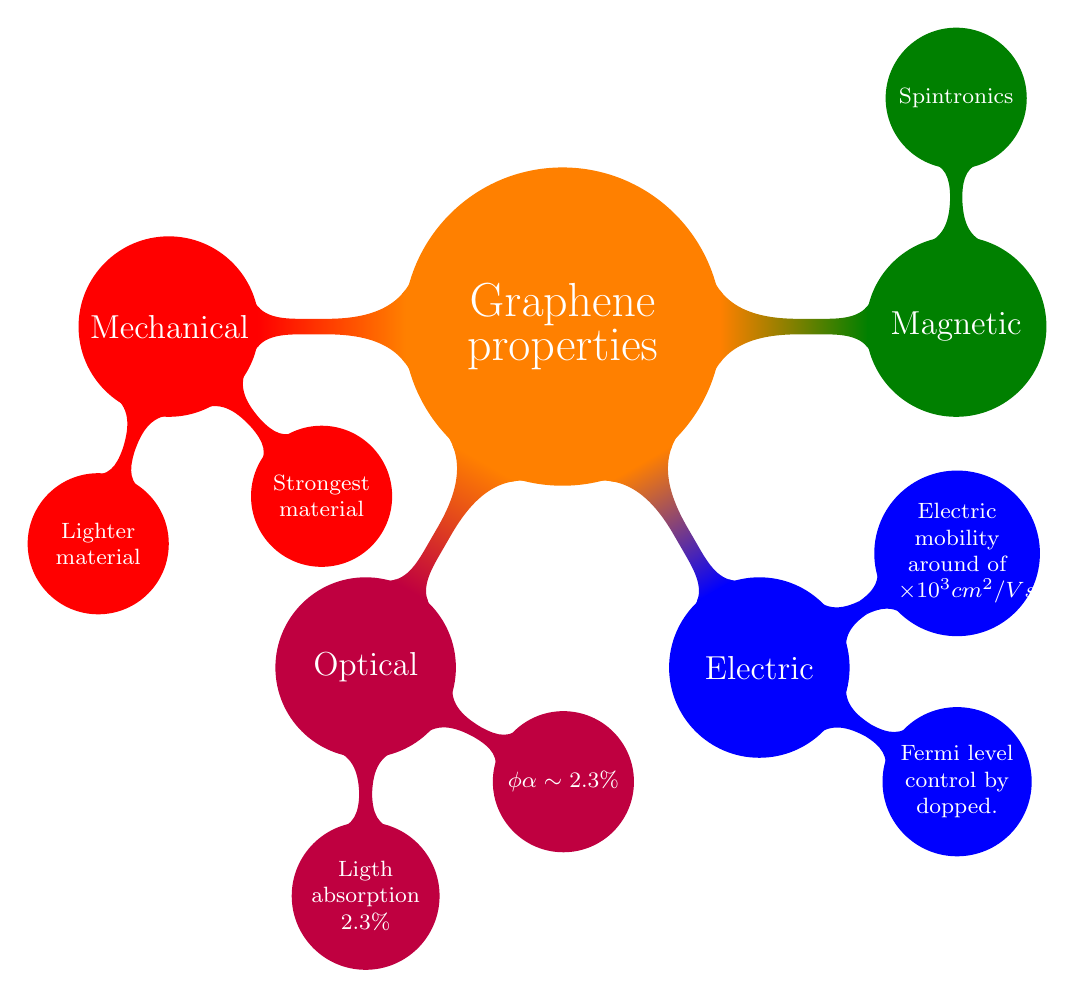
\begin{tikzpicture}
  \path[mindmap,concept color=orange,font=\fontsize{17}{5}\selectfont,text=white]
  node[concept] {Graphene properties}
  [clockwise from=0]
  child[concept color=green!50!black,font=\fontsize{13}{5}\selectfont] {
    node[concept] {Magnetic}
    [clockwise from=90]
    child { node[concept] {Spintronics} }
    %			child { node[concept] {data structures} }
    %			child { node[concept] {pro\-gramming languages} }
  }  
  child[concept color=blue,font=\fontsize{13}{5}\selectfont] {
    node[concept] {Electric}
    [clockwise from=30]
    child { node[concept] {Electric mobility around of $\times10^3 cm^2/V s$} }
    child { node[concept] {Fermi level control by dopped. } }
  }
  child[concept color=purple,font=\fontsize{13}{5}\selectfont] {
    node[concept] {Optical}
    [clockwise from=-30]
    child { node[concept] { $\phi \alpha \sim 2.3 \%$} }
    child { node[concept] {Ligth absorption $2.3\%$} }
  }
  child[concept color=red,font=\fontsize{13}{5}\selectfont] { 
    node[concept] {Mechanical} 
    [clockwise from=-48]
    child { node[concept] {Strongest material} }
    child { node[concept] {Lighter material} }
  }
  ;

% \begin{scope}[opacity=0.3]
%     \draw(0,0) to[labeled grid] (11,11);    
% \end{scope}
        
  \end{tikzpicture}
\end{document}